\documentclass[10pt,a4]{article}
\usepackage[margin=1.3in]{geometry}
\usepackage[UKenglish]{isodate}
% can add citecolor = color below 
\usepackage[colorlinks=true, linkcolor=red, citecolor=black, filecolor=magenta, urlcolor=blue]{hyperref}
\usepackage[T1]{fontenc}
\usepackage{enumitem}
\usepackage{amsmath}
\usepackage{amssymb}
\usepackage{subfigure}
\usepackage{graphicx}
\usepackage{combelow}
\usepackage{cite}
\usepackage[hyphenbreaks]{breakurl}



\usepackage{cleveref}
\crefformat{section}{\S#2#1#3} % see manual of cleveref, section 8.2.1
\crefformat{subsection}{\S#2#1#3}
\crefformat{subsubsection}{\S#2#1#3}

% Custom colors
\usepackage{color}
\definecolor{deepblue}{rgb}{0,0,0.5}
\definecolor{deepred}{rgb}{0.6,0,0}
\definecolor{deepgreen}{rgb}{0,0.5,0}
\definecolor{deeppurple}{rgb}{0.30,0.0,0.15}

\usepackage{hyperref}
\hypersetup{
     colorlinks   = true,
     citecolor    = deepblue,
     linkcolor=deeppurple
}

\usepackage[ruled,commentsnumbered,lined]{algorithm2e} % code
\DontPrintSemicolon

\usepackage{tabu}  % thicker lines in tables
\usepackage{float}
\usepackage{bm}
\usepackage{caption}
\usepackage{listings}
\usepackage{tikz}
%%%%%%%%%%%%%%%%%%%%%%%%%%%%%%%%%%%%%%%%%%%%%%%%%%%%

%%%%%%%%% BAYESIAN DIAGRAMS AND STUFF %%%%%%%%%%%%%%
% tikzlibrary.code.tex
%
% Copyright 2010-2011 by Laura Dietz
% Copyright 2012 by Jaakko Luttinen
%
% The MIT License
%
% See LICENSE file for more details.

% Load other libraries
\usetikzlibrary{shapes}
\usetikzlibrary{fit}
\usetikzlibrary{chains}
\usetikzlibrary{arrows}

% Latent node
\tikzstyle{latent} = [circle,fill=white,draw=black,inner sep=1pt,
minimum size=20pt, font=\fontsize{10}{10}\selectfont, node distance=1]
% Observed node
\tikzstyle{obs} = [latent,fill=gray!25]
% Constant node
\tikzstyle{const} = [rectangle, inner sep=0pt, node distance=1]
% Factor node
\tikzstyle{factor} = [rectangle, fill=black,minimum size=5pt, inner
sep=0pt, node distance=0.4]
% Deterministic node
\tikzstyle{det} = [latent, diamond]

% Plate node
\tikzstyle{plate} = [draw, rectangle, rounded corners, fit=#1]
% Invisible wrapper node
\tikzstyle{wrap} = [inner sep=0pt, fit=#1]
% Gate
\tikzstyle{gate} = [draw, rectangle, dashed, fit=#1]

% Caption node
\tikzstyle{caption} = [font=\footnotesize, node distance=0] %
\tikzstyle{plate caption} = [caption, node distance=0, inner sep=0pt,
below left=5pt and 0pt of #1.south east] %
\tikzstyle{factor caption} = [caption] %
\tikzstyle{every label} += [caption] %

%\pgfdeclarelayer{b}
%\pgfdeclarelayer{f}
%\pgfsetlayers{b,main,f}

% \factoredge [options] {inputs} {factors} {outputs}
\newcommand{\factoredge}[4][]{ %
  % Connect all nodes #2 to all nodes #4 via all factors #3.
  \foreach \f in {#3} { %
    \foreach \x in {#2} { %
      \path (\x) edge[-,#1] (\f) ; %
      %\draw[-,#1] (\x) edge[-] (\f) ; %
    } ;
    \foreach \y in {#4} { %
      \path (\f) edge[->, >={triangle 45}, #1] (\y) ; %
      %\draw[->,#1] (\f) -- (\y) ; %
    } ;
  } ;
}

% \edge [options] {inputs} {outputs}
\newcommand{\edge}[3][]{ %
  % Connect all nodes #2 to all nodes #3.
  \foreach \x in {#2} { %
    \foreach \y in {#3} { %
      \path (\x) edge [->, >={triangle 45}, #1] (\y) ;%
      %\draw[->,#1] (\x) -- (\y) ;%
    } ;
  } ;
}

% \factor [options] {name} {caption} {inputs} {outputs}
\newcommand{\factor}[5][]{ %
  % Draw the factor node. Use alias to allow empty names.
  \node[factor, label={[name=#2-caption]#3}, name=#2, #1,
  alias=#2-alias] {} ; %
  % Connect all inputs to outputs via this factor
  \factoredge {#4} {#2-alias} {#5} ; %
}

% \plate [options] {name} {fitlist} {caption}
\newcommand{\plate}[4][]{ %
  \node[wrap=#3] (#2-wrap) {}; %
  \node[plate caption=#2-wrap] (#2-caption) {#4}; %
  \node[plate=(#2-wrap)(#2-caption), #1] (#2) {}; %
}

% \gate [options] {name} {fitlist} {inputs}
\newcommand{\gate}[4][]{ %
  \node[gate=#3, name=#2, #1, alias=#2-alias] {}; %
  \foreach \x in {#4} { %
    \draw [-*,thick] (\x) -- (#2-alias); %
  } ;%
}

% \vgate {name} {fitlist-left} {caption-left} {fitlist-right}
% {caption-right} {inputs}
\newcommand{\vgate}[6]{ %
  % Wrap the left and right parts
  \node[wrap=#2] (#1-left) {}; %
  \node[wrap=#4] (#1-right) {}; %
  % Draw the gate
  \node[gate=(#1-left)(#1-right)] (#1) {}; %
  % Add captions
  \node[caption, below left=of #1.north ] (#1-left-caption)
  {#3}; %
  \node[caption, below right=of #1.north ] (#1-right-caption)
  {#5}; %
  % Draw middle separation
  \draw [-, dashed] (#1.north) -- (#1.south); %
  % Draw inputs
  \foreach \x in {#6} { %
    \draw [-*,thick] (\x) -- (#1); %
  } ;%
}

% \hgate {name} {fitlist-top} {caption-top} {fitlist-bottom}
% {caption-bottom} {inputs}
\newcommand{\hgate}[6]{ %
  % Wrap the left and right parts
  \node[wrap=#2] (#1-top) {}; %
  \node[wrap=#4] (#1-bottom) {}; %
  % Draw the gate
  \node[gate=(#1-top)(#1-bottom)] (#1) {}; %
  % Add captions
  \node[caption, above right=of #1.west ] (#1-top-caption)
  {#3}; %
  \node[caption, below right=of #1.west ] (#1-bottom-caption)
  {#5}; %
  % Draw middle separation
  \draw [-, dashed] (#1.west) -- (#1.east); %
  % Draw inputs
  \foreach \x in {#6} { %
    \draw [-*,thick] (\x) -- (#1); %
  } ;%
}

%%%%%%%%%%%%%%%%%%%%%%%%%%%%%%%%%%%%%%%%%%%%%%%%%%%%%





\cleanlookdateon

\begin{document}
\bibliographystyle{plain}

\thispagestyle{empty}

\newcommand{\HRulee}{\rule{\linewidth}{0.5mm}}

\vfil

{\raggedleft \large Razvan Kusztos \\}
{\raggedleft \large Girton College \\}
{\raggedleft \large \tt rek43@cam.ac.uk \\}

\vspace{50pt}

\begin{center}

	{\Large \sc Computer Science Tripos, Part III \\}
	\vspace{10pt}
	{\Large \sc LE49: Probabilistic Machine Learning\\}
	\vspace{20pt}
	\HRulee \\[0.1cm]
	\vspace{10pt}
	{\LARGE \bf Dota2 Player Ranking Using Trueskill\texttrademark}
	\HRulee \\[20pt]
	{\LARGE  Report\\}
	\vspace{20pt}
	{\Large \today \\}
	\vspace{40pt}
\end{center}

\vfill

\begin{flushright}
%TODO: add wordcount
Word count: 2630
\end{flushright}
	
\newpage

\section{Introduction}

Player ranking has many important uses in competitive sports or games. Firstly, 
they provide a basis to matchmaking systems, improving the experiences of both 
players and watchers. They create balanced games for the participants, while 
keeping them dynamic for audiences. Secondly, ranking players can be used to determine 
tournament qualification (such as the access to ranked matches in Dota2). Lastly, 
ranking triggers the human ingrained response to competition, attracting players 
to stay for longer, thus benefiting the industry.

The essence of ranking algorithms is determining a real skill score for each 
player, such that its magnitude is representative of the player's future 
performances. In a probabilistic setting, these skills must also be depictive of 
the probability of future games' outcome.

One of the most influential statistical ranking systems is due to Arpad Elo (1959) 
\cite{elo1978rating}, and has been used extensively in chess ranking 
\cite{glickman1995comprehensive}. In the online game scene, it has been used in 
World of Warcraft's PvP\footnote{player vs. player} matchmaking 
\footnote{\url{http://wowwiki.wikia.com/wiki/Arena_personal_rating}}. 

The core of the \emph{Elo} algorithm is that each player's game performance  
is normally distributed around their skill, $p \sim \mathcal{N}(skill, \beta^2)$.
The probability that one player wins is then proportional to the probability that 
its performance is higher than its adversary's.
\begin{align*}
	P(p_1 > p_2 | skill_1, skill_2) = \Phi\bigg(\frac{s_1 - s_2}{\sqrt{2}\beta}\bigg),
\end{align*}
where $\Phi$ is the cumulative density of a normalised Gaussian distribution. 


The \emph{Glicko} rating systems \cite{glickman1999parameter}, \cite{glickman2012example}. 
were introduced as improvements to \emph{Elo}. 
They replace the constant variance parameter used by the
\emph{Elo} system by shifting to a Bayesian framework. In this setting, the player skill itself 
is modelled as a sample from a prior distribution and, with each game, the uncertainty 
(variance) we hold about their skill decreases. 

Unfortunately \emph{Glicko} is limited to single player games. Microsoft 
TrueSkill\texttrademark  was developed to address this limitation, by allowing 
individuals' skills to be updated given the team's performance, as well as considering
games with more than 2 competing entities.

An important question that needs yet to be addressed is how to enhance these existing
systems by incorporating other information about the players, rather than just 
win vs. loss information. For instance, in chess, one might incorporate knowledge of whether 
the player controls the black or the white. 
A way in which this problem has been addressed is due to \emph{Zhang et al.} 
\cite{zhang2010factor}. They suggested that a skill, rather than being 
a single real value, could be modelled as a vector of skill components: \emph{
a virtual team of [the player's] various skills}. Of particular interest to the 
current work is that they validate their algorithm on \emph{DotA}, a precursor of 
the game I will discuss in this work.


In the rest of this report, I will introduce factor graphs and the message passing 
algorithms, necessary for understanding the \emph{TrueSkill\texttrademark}
original implementation. I will then describe the assumptions made in the 
\emph{TrueSkill\texttrademark} model. Next, I will introduce the particularities 
of the \emph{Dota2} game, a multiplayer online battle arena (MOBA) that has been 
part of the recent advent of e-sports. Lastly, I incorporate these considerations 
into an implementation that I evaluate on both real and synthesized datasets.

\section{Implementation} \label{impl}

\subsection{Factor Graphs}

The \emph{Factor Graph} is a graph-based graphical model. Like \emph{Markov Random Fields}
or \emph{Bayesian Networks}, it is used to model multivariate probability distribution 
while making explicit the conditional independence assumptions of the random variables.
The \emph{Factor Graph} is based on a bipartite undirected graph with two types of nodes:
\textbf{variables} (depicted as circles), and \textbf{factors} (depicted as squares).
The factors represent functorial combinations of the neighbouring variables. The 
bipartite structure is achieved by enforcing the constraint that edges can only
connect nodes of different types.

Another way to see it is that the factor graph expresses a factorisation of a 
joint distribution:

\begin{align*}
	g(x_1, x_2, x_3, ..., x_n)=\sum_{j \in J}f_j(\textbf{x}_j),
\end{align*}
where $J$ is the set of factors and $\textbf{x}_j$ is the list of variables that 
are adjoint to the node representing the factor $f_j$.

We are generally interested in performing marginalisation. This is usually 
required in practice, for example when computing likelyhood functions.

\begin{align*}
	g_i(x_i) = \sum_{x_j, j \neq i}g(x_1, x_2, ..., x_n)
\end{align*}

\subsection{Message Passing}

Marginalisation approximations are performed using the so called \emph{sum-product algorithm}. 
Also known as \emph{Belief propagation}\cite{pearl1982reverend}, this algorithm was designed
to be a general, easily parallelisable, exact inference of graphical model
based on trees. However, it is known to provide approximations on general graphs
\cite{pearl2014probabilistic}, including cyclic graphs \cite{murphy1999loopy}.

It has been shown that this algorithm is an instance of the 
\emph{Expectation propagation}\cite{minka2001expectation} on factor graphs. 
The algorithm approximates marginals by propagating \emph{messages} along the 
edges of the factor graphs. In the context of \emph{Expectation propagation}, 
messages are nothing but factor approximations obtained in the main loop of the 
algorithm \cite{minka2001expectation}.

Concretely, message passing can be defined through the following equations:
\begin{align*}
	p(v_i) &= \prod_{f \in {F_{v_i}}}m_{f \to v_i}(v_i)  \\
	m_{f \to v_i}(v_i) &= \int...\int f(\textbf{v}) \prod_{i \neq j}m_{v_j \to f}(v_i)dv_j \\
	m_{v_i \to f}(v_i) &= \frac{p(v_i)}{m_{f \to v_i}} 
\end{align*}
In the previous, $f$ refers to a factor and $v$ to a variable node. I use the 
standard notation $m_{f \to v}$ to represent the message from node $f$ to node $v$.

\subsection{TrueSkill Implementation}

For simplification, I will introduce this problem with no-draw games consisting 
of two teams, each with two players. 

We model all players' skills as being drawn from a prior normal distribution. This encodes
the knowledge we have about the players before beginning to analyse their game 
outcomes. Then, we calculate the team performance as being the sum of the 
members' skills with an added \emph{Gaussian noise}, representing a \emph{luck}
element. Lastly, the probability of the team winning is given by the probability 
the first team's performance is higher than the second team's performance

\begin{figure}[ht]
	\begin{center}
	  	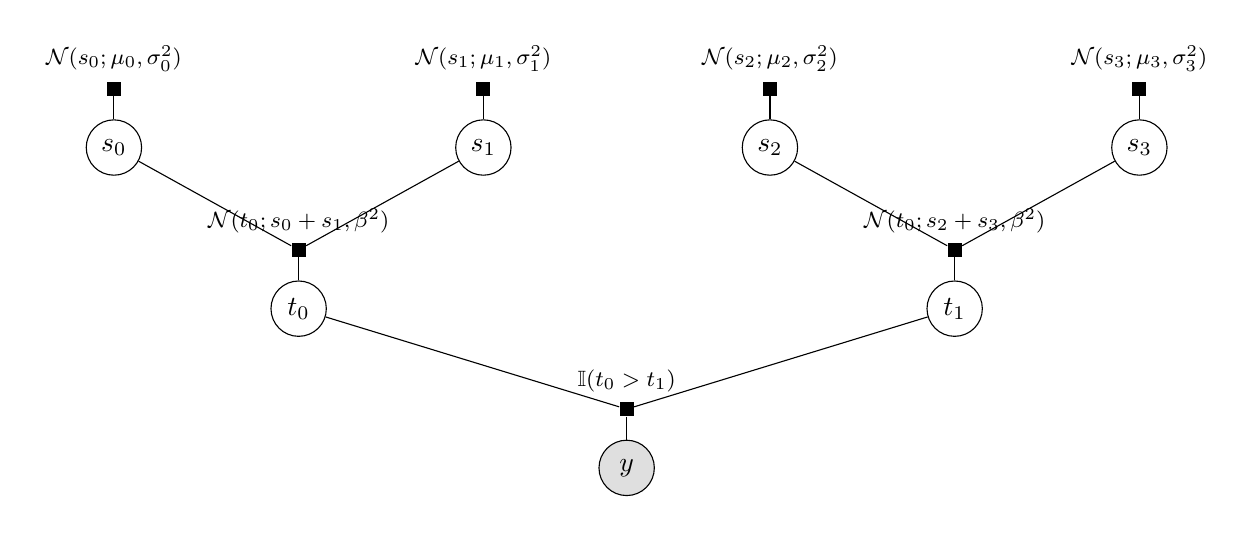
\begin{tikzpicture}[x=1.0cm,y=1.0cm]

	\matrix[row sep=0.3cm, column sep=0.1cm] (LDA)
	{ %
	  \factor      {prior0}  {$\mathcal{N}(s_0; \mu _0, \sigma _0^2)$} {} {}; & &
	  \factor      {prior1}  {$\mathcal{N}(s_1; \mu _1, \sigma _1^2)$} {} {}; & &
	  \factor      {prior2}  {$\mathcal{N}(s_2; \mu _2, \sigma _2^2)$} {} {}; & &
	  \factor      {prior3}  {$\mathcal{N}(s_3; \mu _3, \sigma _3^2)$} {} {};  
	  \\
	  \node[latent] (skill0)  {$s_0$} ; & & 
	  \node[latent] (skill1)  {$s_1$} ; & &
	  \node[latent] (skill2)  {$s_2$} ; & &
	  \node[latent] (skill3)  {$s_3$} ;
	  \\
	  & %
	  \factor       {team0}   {$\mathcal{N}(t_0; s_0 + s_1, \beta ^2)$} {} {}; & & & & %
	  \factor       {team1}   {$\mathcal{N}(t_0; s_2 + s_3, \beta ^2)$} {} {}; & %
	  \\
	  &
	  \node[latent] (performance0)   {$t_0$} ; & & & & %
	  \node[latent] (performance1)   {$t_1$} ; & %
	  \\
	  & & & %
	  \factor       {cutout}   {$\mathbb{I}(t_0 > t_1)$} {} {}; %
	  \\
	  & & & 
	  \node[obs] (outcome)   {$y$} ;  %
	  \\
	};
  
	\factoredge {prior0} {skill0} {};
	\factoredge {prior1} {skill1} {};
	\factoredge {prior2} {skill2} {};
	\factoredge {prior3} {skill3} {};
		
	\factoredge {skill0, skill1} {team0} {};
	\factoredge {skill2, skill3} {team1} {};

	\factoredge {team0} {performance0} {};
	\factoredge {team1} {performance1} {};

	\factoredge {performance0, performance1} {cutout} {};

	\factoredge {cutout} {outcome} {};

\end{tikzpicture}	

	\end{center}
	\caption{Original TrueSkill\texttrademark  model for a game with two teams of
	two members each. Note that, in the above, I only show a small part of the full graph, 
	related to a single game. In reality, we have $N$ players and $G$ games.
	}
	\label{fig:stdts}
\end{figure}

We are interested in computing the marginal distribution, 
$
\mathbb{P}(s_i | \mathbf{s}, \mathbf{t}, \mathbf{y})
$ for each player $i$. We can do these by applying the sum product algorithm. 
The derivation of the message passing equation is an exercise in \emph{Gaussian}
distribution manipulations \cite{herbrich2007trueskill}. 
Notice however that we need to make two further approximations. 

Firstly, because 
of the presence of cyclic structures (since the same player can take part in 
multiple games), we will have to make use of the \emph{loopy belief propagation}
ideas and iterate a few times through the steps of the algorithm. 

Secondly, the 
efficiency of \emph{expectation propagation} is due to the small amount of moments 
that we need to to propagate through the network. In the case of the \emph{normal distribution}, two moments
suffice ($\mu$ and $\sigma$). However, for the factor computing $\mathbb{I}(t_0 > t_1)$,
we can apply \emph{moment matching} to approximate its result to a \emph{Gaussian}. 
This reduces to applying \emph{moment matching} on a truncated \emph{Gaussian}, say:
$t \sim \frac{1}{Z_t}\delta (t > 0) \mathcal{N}(t; \mu ,\sigma ^2)$. By using the 
notation:
\begin{align*}
	\Psi(z) &= \frac{\mathcal{N}(z;0, 1)}{\Phi(z)} \\
	\Lambda(z) &= \Psi(z)(\Psi(z) + z), \\
\intertext{We can approximate the distribution of $t$ by a Gaussian whose moments 
are \footnotemark:} 
	\mathbb{E}(t) &= \mu + \sigma\Psi(\frac{\mu}{\sigma}) \\ 
	\text{Var}(t) &= \sigma ^ 2 (1 - \Lambda(\frac{\mu}{\sigma}))
\end{align*}
\footnotetext{\url{http://mlg.eng.cam.ac.uk/teaching/4f13/1718}}

Notice that under this model, the only factors that are open to modification are  
the prior distribution of the skills and the outcome of the game. There is no other
way to incorporate new assumptions that are valid in particular games we apply
this model to.
In the following, I will present a few simple modification that could better
fit the game of DotA2, as well as validate them on synthesized and real datasets.

\subsection{DotA2}

Dota2 (Defense of the Ancients 2) is a Multiplayer Online Battle Arena(MOBA). 
The \emph{Arena} is a square map 
containing two adversary bases on opposite corners, united by three lanes heavily
guarded by turrets. There are two teams, referred to as the \emph{Radiance} and \emph{Dire},
each of which is composed of five human players. The goal of a team is to infiltrate 
the enemy base and destroy their \emph{Ancient}, a static structure. Upon achieving
this feat, the game terminates.

Each human player controls a \emph{hero} which they can chose before the game commences.
The \emph{heroes} are all different, requiring particular strategies. During 
clashes between teams, \emph{heroes} might get killed, which confers their slayers
\emph{gold} and \emph{experience}. Upon death, \emph{heroes} \emph{respawn} after 
a penalty time during which the player can only observe the game. 

Although this is an incomplete description of the game\footnote{\url{https://dota2.gamepedia.com/Dota_2_Wiki}}
, it suffices for understanding the metrics provided by specialised datasets, such as: 
duration of the game, hero name, kills, deaths, gold per minute, xp per minute etc.

\subsubsection{Dota2 Ranking Dataset.}

For running experiment in following sections, I will be using a \emph{Kaggle}-hosted
dataset \footnote{\url{https://www.kaggle.com/owajawa/dota-2-skill-rating-with-trueskill/data}},
created by querying the OpenDota service \footnote{\url{https://www.opendota.com/}}.
This dataset contains metadata about matches (e.g. duration, geographic information),
as well as some of the players that took part in it (e.g. level, experience, 
gold, damage dealt, the hero chosen, deaths, kills etc.). Furthermore, it contains
timestamps of all the events that took part in the game, such as items bought, 
and even the text log. As the data is very rich, constructing a probabilistic model
that integrates all these variables would require some amount of domain knowledge. 
Nonetheless, in the next sections, I will outline a few assumptions that we can
check about the data. 

\subsection{Assumptions about the data}

\subsubsection{Matchmaking bias}
The platform implements a matchmaking routine \footnote{\url{https://dev.dota2.com/showthread.php?t=129665}}.
Also based on a probabilistic assumption, their algorithm assigns skill levels,
called MMR - Match Making Rating. This number, originally starting at the value of 
3000 is increased with every win and decreased with every loss. The difference depends
on the MMR difference between the two teams. 

Players will only play games with peers of a similar skill. This contradicts the 
independence assumption between the players. 

It is worth noting that the data does not account for the entire history of all 
the players that occur in the present matches. This makes simple heuristics for 
approximating skills uninteresting, such as the simple win/loss ratio. However, 
we can still observe the matchmaking bias by analysing some other features of the 
players, such as their gold per minute or xp per minute gains. These numbers are 
more likely to be representative of the player's skill. A visualisation of the  
the bias is shown in Figure \ref{fig:differences}. The relatively low shift 
is possibly due to a selection bias in the data, by picking all matches to be in 
the same league.

\begin{figure}[h!]
  \centering
  \mbox{
      \subfigure{
          \includegraphics[width=0.4\textwidth]{../dota_rank/vis/gpm.png}
      }\quad
      \subfigure{
          \includegraphics[width=0.4\textwidth]{../dota_rank/vis/xpm.png}
          }
  }
  \mbox{
  \subfigure{
    \includegraphics[width=0.4\textwidth]{../dota_rank/vis/win_ratio.png}
    }
  }
  \caption{Graphs showing the range of values in standard deviations of player
  metrics, computed in the context of individual matches. 
  The blue line corresponds to the actual data, whereas the gray line is obtained 
  assigning the players randomly to matches, mimicking a random dataset.
  The first two plots show \emph{gold per minute} and \emph{xp per minute}, 
  illustrating the bias in the real data. The last plot shows \emph{win ratio}.}
  \label{fig:differences}
\end{figure}

\subsubsection{Anonymous players}
A substantial amount of players choose to play anonymously, accounting to 
more than 99\% of matches. In this case, the system does not preserve any 
identification that could trace back the individual from the gameplay information. 
This turns out to be a critical problem in modeling the calculation of 
\emph{team performances}.

As a preprocessing step, I decide to ignore the matches containing teams with less
than two non-anonymous players. Then, I modify the calculation of the team 
performances to be the mean of the skills of non-anonymous players. This is 
consistent with the assumption that peers are close in skills. 

\subsubsection{Analysis of feature importance}
\label{sssec:features}

The feature space of the players is relatively big, given the sparsity of the data.
We can therefore employ supervised techniques for picking only the most important ones.
Inspired from the work of \emph {I. Guyon et al.} \cite{guyon2002gene}, we can 
pose the problem as an instance of a supervised machine learning task and solve it 
using linear SVM. The relative coefficients of the features could be representative 
of feature importance (the original paper uses the square of these values).

The problem could be posed as a supervised learning problem, we can split the 
match history into \emph{past} and \emph{future}. Taking the features of players
analysed in the \emph{past} can be used to infer the match results in the \emph{future}.

\begin{figure}[h!]
  \centering
  \mbox{
      \subfigure{
          \includegraphics[width=0.4\textwidth]{../dota_rank/vis/download.png}
  }
  }
  \caption{
    This plot presents the relative importance of the features, as explained in 
  section \ref{sssec:features}. This clasifier obtained a 
  low score, but nonetheless better than random. I tried linear SVM (51.8\%) and 
  RBF SVM (54.0\%)
  }
  \label{fig:feature_imp}
\end{figure}

\section{Results}

\subsection{Synthesized dataset}

In order to validate the implementation of the algorithm, I have used a simple,
synthesized dataset. This is generated by first picking the \emph{team performance}
and then forming teams of players whose skills are close in magnitude to the 
team performance. 

Making a synthesized dataset to capture the richness of the 
players' features would require specialised knowledge, so this dataset is being 
used solely to validate implementations of the baseline algorithms.

\subsection{Baseline results}
\label{ssec:baseline}
An important step toward integrating the features into calculation is determining 
the predictive power of the wins and loss history. From the results, I deduce 
that the statement of the problem of ranking as a supervised machine 
learning task requires extra thought. During these experiments, I have split the 
match history into \emph{training} (80\%) and \emph{testing} (20\%). \emph{Elo} and \emph{Trueskill}
scores were inferred for players that took part in the training matches. The reported 
results are the percentage of games in the testing matches whose outcome was 
correctly predicted, using the players' scores from the previous steps. Players 
whose scores were not computed in the training phase were replaced with anonymous 
players. The results are shown in Table \ref{tab:results}.

In all the future results, the accuracies given are the result of averaging a set 
of N=5 results, to account for the random components of the algorithm.


\begin{table}[h!]
  \centering
  \begin{tabular}{l l c}
    \textbf{Algorithm} & \textbf{Dataset} &  \textbf{Accuracy} \\ 
    \hline
    Linear SVM         & Real             &  51.8\% \\
    \hline
    Elo                & Real             &  52.4\% \\
    Elo                & Synth            &  55.4\% \\
    \hline
    Trueskill (lib)    & Real             &  51.0\% \\
    Trueskill (lib)    & Synth            &  54.3\% \\
    \hline
    Trueskill (imp)    & Real             &  51.2\% \\
    Trueskill (imp)    & Synth            &  55.4\% \\    
    \hline 
  \end{tabular}
  \caption{Summary of \emph{baseline} results. Trueskill (lib) is using the 
  a python library(\url{http://trueskill.org/}), based on an online learning scheme 
  via \emph{Gaussian density filtering}\cite{minka2001expectation}. My implementation
  is inspired from \url{http://mlg.eng.cam.ac.uk/teaching/4f13/1718/}, only made 
  more efficient by using sparse matrices. The Elo implementation is inspired from 
  \url{https://www.kaggle.com/kplauritzen/elo-ratings-in-python}}.   
  \label{tab:results}
\end{table}

\begin{figure}[h!]
  \centering
  \mbox{
      \subfigure{
          \includegraphics[width=0.4\textwidth]{../dota_rank/vis/impvelo.png}
      }\quad
      \subfigure{
          \includegraphics[width=0.4\textwidth]{../dota_rank/vis/impvlib.png}
          }
  }
  \caption{Figures showing the correlation between skills computed by the three 
  presented algorithms, indicating a degree of equivalence.}
\end{figure}


\subsection{Integrating numeric features}

Although the SVM was not capable of extracting more information from the features, 
it was worth trying integrating this information in the probabilistic model. 
To this end, I suggest two possibilities:
\begin{itemize}
  \item Using the relative magnitude of each players' features as part of the prior
  \item Training an alternative model that considers as winners the team with the 
  bigger mean feature. 
\end{itemize}
The results are presented in Table \ref{tab:features}.

\begin{table}[h!]
  \centering
  \begin{tabular}{l c}
    \textbf{Feature} & \textbf{Accuracy} \\
    \hline
    \emph{gold per minute} & 51.7\% \\ 
    \emph{kills / deaths} & 51.1\% \\
    \emph{(kills + assists)/deaths} & 51.5\% \\
    \emph{gold spent} & 51.9\% \\
    \hline
  \end{tabular}
  \quad
  \begin{tabular}{l c}
    \textbf{Feature} & \textbf{Accuracy} \\
    \hline
    \emph{gold spent} & 49.9\% \\
    \emph{gold per min} & 50.0\% \\
    \emph{kills} & 49.9\% \\
    \emph{assists} & 50.9\% \\
    \hline 
  \end{tabular}
  \caption{Summary of the results by integrating features. On the left, I present 
  the results when feature information is added to the prior of the skills. On the 
  right, I show the variant of pretraining the model based on feature information,
  and then using the results skills as priors.}
  \label{tab:features}
\end{table}

\subsubsection{Integrating Hero information}
\label{sssec:hero}
In order to integrate hero information, I suggest considering players as virtual
teams containing the human component and the hero. In order to simplify the model, 
I first calculate the \emph{skills} of heroes, simply by replacing the player ids 
with the hero ids in the TrueSkill algorithm. Then, I average this value with the 
value of skills computed as in the baseline in Section \ref{ssec:baseline}. This 
final value is used for predicting future games. The results could be seen in 
Table \ref{tab:hero}.

\begin{table}[h!]
  \centering
  \begin{tabular}{l l}
    \textbf{Model} & \textbf{Accuracy} \\
    \hline
    \emph{Baseline Trueskill} & 51.2\% \\ 
    \emph{Hero Trueskill} & 54.2\%($\pm$0.8\%) \\
    \hline
  \end{tabular}
  \caption{Comparing the results of the baseline and those of the algorithm that 
  integrates hero information}
  \label{tab:hero}
\end{table}

\section{Conclusions}

In this project, I attempted to illustrate benefits of integrating the richness of 
of player's previous gameplay information in a standard, probabilistic machine learning 
algorithm. In particular, the hero information seemed to be the most fruitful (Section \ref{sssec:hero}).

On main point that came across during the experiments was the difficulty of posing
this problem as a supervised machine learning problem. The TrueSkill algorithm 
under-performed in all models, including when run on synthesized datasets. There
seems to be a fundamental problem in extrapolating training data to testing data, 
obtaining scores only marginally higher than random. However, in the case of 
synthesized datasets, the algorithms' scores were capable of obtaining training accuracies 
one standard deviation away from the scores obtained with the truth values. 
This could possibly hint at the need of introducing more regularisation techniques,
perhaps bespoke variance terms when computing team performance for each player.
More generally, exploring how to better pose this problem in a supervised 
setting is potentially a good start for future work.

A second problem was that due to the little amount of data and high variability of 
the players, the true advantage of using a probabilistic framework could not be 
explored. The variances were often trumping the means in absolute magnitude, making
it hard to view the results in a probabilistic mindset. By exploring correlations 
between the players rating and their features, assuming access to more data, we could 
potentially in future work use variance reduction techniques, such as using 
control variates in a MCMC formulation of TrueSkill.















































 
\newpage
\bibliography{references}
\end{document}
